\clearpage

\subsection{Translucent without Survivability}\label{ILP_Transluc_Survivability}
\begin{tcolorbox}	
\begin{tabular}{p{2.75cm} p{0.2cm} p{10.5cm}} 	
\textbf{Student Name}  &:& Tiago Esteves    (October 03, 2017 - )\\
\textbf{Goal}          &:& Implement the ILP model for the translucent transport mode without survivability.
\end{tabular}
\end{tcolorbox}

\subsubsection{Model description}

First, for a better understanding of the functions and variables used in the ILP, a table \ref{description_transluc} will be created with all indexes, inputs and variables and with their respective description.

\begin{table}[h!]
\centering
\begin{tabular}{ |p{1cm}||p{13cm}|}
 \hline
 \multicolumn{2}{|c|}{Description of notation used in the objective function} \\
 \hline
 \hline
 $i$ & index for start node of a physical link \\
 $j$ & index for end node of a physical link \\
 $o$ & index for node that is origin of a demand \\
 $d$ & index for node that is destination of a demand \\
 $c$ & index for bit rate of the client signal \\
 $($ i,j $)$ & physical link between the nodes $i$ and $j$ \\
 $($ o,d $)$ & demand between the nodes $o$ and $d$ \\
 $C$ & set of the client signal \\
 $L_{ij}$ & binary variable indicating if link between the nodes $i$ and $j$ is used \\
 $Ls_{ij}^{od}$ & Number of ODU-o low speed signals from node $o$ to node $d$ employing lightpath ($i$,$j$) \\
 $f_{ij}^{od}$ & Number of 100 Gbit/s optical channels (number of flows) between the link $i$ and $j$ for all demand pairs between $o$ and $d$ \\
 $\lambda_{od}$ & Number of lightpath channels between the nodes $o$ and $d$ \\
 $B$ & Client signals granularities $($1.25, 2.5, 10, 40, 100$)$ \\
 $D_{odc}$ & Client traffic demands between the nodes $o$ and $d$ with bit rate $c$ \\
 $G$ & Network topology in form of adjacency matrix \\
 \hline
\end{tabular}
\caption{Table with description of variables}
\label{description_transluc}
\end{table}

Before carrying out the description of the objective function we must take into account the following particularity of this mode of transport:
\begin{itemize}
  \item $N_{OXC,n}$ = 1, \quad $\forall$ n that process traffic
  \item $N_{EXC,n}$ = 1, \quad $\forall$ n that process traffic
\end{itemize}

\vspace{7pt}
The objective function of following the ILP is a minimization of the CAPEX through the equation \ref{Capex} where in this case for the cost of nodes we have in consideration electric \ref{Capex_Node_EXC} and optical cost \ref{Capex_Node_OXC}. In this case the value of $P_{exc,c,n}$ is obtained by equation \ref{EXC_pexc1_transluc} for short-reach and by the equation \ref{EXC_pexc2_transluc} for long-reach and the value of $P_{oxc,n}$ is obtained by equation \ref{OXC_poxc_transluc}.\\

The equation \ref{EXC_pexc1_transluc} refers to the number of sort-reach ports of the electrical switch with bit-rate $c$ in node $n$, $P_{exc,c,n}$, i.e. the number of tributary ports with bit-rate $c$ in node $n$ which can be calculated as

\begin{equation}
P_{exc,c,n} = \sum_{d=1}^{N} D_{nd,c}
\label{EXC_pexc1_transluc}
\end{equation}

\vspace{11pt}
\noindent
where $D_{nd,c}$ are the client demands between nodes $n$ and $d$ with bit rate $c$.\\

In this case there is the following particularity:
\begin{itemize}
  \item When $n$=$d$ the value of client demands is always zero, i.e, $D_{nn,c}=0$
\end{itemize}

\vspace{11pt}
As previously mentioned, the equation \ref{EXC_pexc2_transluc} refers to the number of long-reach ports of the electrical switch with bit-rate -1 in node n, $P_{exc,-1,n}$, i.e. the number of add ports of node n which can be calculated as

\begin{equation}
P_{exc,-1,n} = \sum_{j=1}^{N} \lambda_{nj}
\label{EXC_pexc2_transluc}
\end{equation}

\vspace{11pt}
\noindent
where $\lambda_{nj}$ is the number of optical channels between node $n$ and node $j$.\\

The equation \ref{OXC_poxc_transluc} refers to the number of ports in optical switch in node n, $P_{oxc,n}$, i.e. the number of line ports and the number of adding ports of node n which can be calculated as

\begin{equation}
P_{oxc,n} = \sum_{j=1}^{N} f_{nj}^{od} + \sum_{j=1}^{N} \lambda_{nj}
\label{OXC_poxc_transluc}
\end{equation}

\vspace{11pt}
\noindent
where $f_{nj}^{od}$ refers to the number of line ports for all demand pairs (od) and $\lambda_{nj}$ refers to the number of add ports.\\

The objective function, to be minimized, is the expression \ref{ILPOpaque_CAPEX}, i.e.,
\begin{equation*}
  minimize \qquad \Big\{ \quad C_C \quad \Big\}
\end{equation*}

$subject$ $to$
\begin{equation}
\sum_{j\textbackslash \{o\}} Ls_{ij}^{odc} = D_{odc}  \qquad \qquad \qquad \qquad \qquad \qquad \qquad \qquad \qquad
\forall(o,d) : o < d, \forall i: i = o
\label{ILPTransluc1}
\end{equation}
\noindent
This constraint are the virtual flow conservation constraints and ensure that, for all (o,d) pairs with bit rate $c$ we routes client demand traffic of flow from node $o$ to node $d$ with bit rate $c$ for all bidirectional links (i,j) when $j$ is not equal to the origin of the demand.

\begin{equation}
\sum_{j\textbackslash \{i,o\}} Ls_{ij}^{odc} = \sum_{j\textbackslash \{i,d\}} Ls_{ji}^{odc} \qquad \qquad \qquad \qquad \qquad \qquad \qquad
\forall(o,d) : o < d, \forall i: i \neq o,d
\label{ILPTransluc2}
\end{equation}
\noindent
In this constraint, assuming bidirectional traffic, so the demand traffic of flow in both directions of the link is the same.

\begin{equation}
\sum_{j\textbackslash \{d\}} Ls_{ji}^{odc} = D_{odc} \qquad \qquad \qquad \qquad \qquad \qquad \qquad \qquad \qquad
\forall(o,d) : o < d, \forall i: i = d
\label{ILPTransluc3}
\end{equation}
\noindent
This constraint are the virtual flow conservation constraints and ensure that, for all (o,d) pairs with bit rate $c$ we routes demand traffic of flow from node $o$ to node $d$ with bit rate $c$ for all bidirectional links (j,i) when $i$ is not equal to the destination of the demand.

\begin{equation}
\sum_{o=1} \sum_{d=o+1} B(c) Ls_{ij}^{odc} \leq  \tau \lambda_{od} \qquad \qquad \qquad \qquad \qquad \qquad \qquad \qquad \qquad \qquad
\forall (i,j)
\label{ILPTransluc4}
\end{equation}
\noindent
This restriction is considered grooming constraint and the variable $\tau$ is always 100 Gbits/s.

\begin{equation}
\sum_{j\textbackslash \{o\}} f_{ij}^{od} = \lambda_{od}  \qquad \qquad \qquad \qquad \qquad \qquad \qquad \qquad \qquad
\forall(o,d) : o < d, \forall i: i = o
\label{ILPTransluc6}
\end{equation}
\noindent
This constraint are equal to the constraint \ref{ILPOpaque1_CAPEX} assuming that Z variable has the value of number of optical channels between this demand for all bidirectional links.

\begin{equation}
\sum_{j\textbackslash \{o\}} f_{ij}^{od} = \sum_{j\textbackslash \{d\}} f_{ji}^{od} \qquad \qquad \qquad \qquad \qquad \qquad \qquad \qquad
\forall(o,d) : o < d, \forall i: i \neq o,d
\label{ILPTransluc7}
\end{equation}
\noindent
This constraint are equal to the constraint \ref{ILPOpaque2_CAPEX}.

\begin{equation}
\sum_{j\textbackslash \{d\}} f_{ji}^{od} = \lambda_{od}  \qquad \qquad \qquad \qquad \qquad \qquad \qquad \qquad \qquad
\forall(o,d) : o < d, \forall i: i = d
\label{ILPTransluc8}
\end{equation}
\noindent
This constraint are equal to the constraint \ref{ILPOpaque3_CAPEX} assuming that Z variable has the value of number of optical channels between this demand for all bidirectional links.

\begin{equation}
\sum_{o=1} \sum_{d=o+1} \left( f_{ij}^{od} + f_{ji}^{od}\right) \leq K_{ij} G_{ij} L_{ij} \qquad \qquad \qquad \qquad \qquad \qquad \qquad
\forall (i,j) : i < j
\label{ILPTransluc9}
\end{equation}
\noindent
This restriction answers capacity constraint problem. Then, total flows must be less or equal to the capacity of network links. For any situation the maximum number of optical channels supported by each transmission system is 100, i.e., $K_{ij}$ = 100.

\begin{equation}
f_{ij}^{od} , f_{ji}^{od} , Ls_{ij}^{odc} , Ls_{ji}^{odc} , \lambda_{od} \in \mathbb{N}   \qquad \qquad \qquad \qquad \qquad
\forall(i,j) : i < j, \forall(o,d) : o < d
\label{ILPTransluc10}
\end{equation}
\noindent
This constraint defines that these variables must be a counting number.

\begin{equation}
L_{i,j} \in \{0,1\} \qquad \qquad \qquad \qquad \qquad \qquad \qquad \qquad \qquad \qquad \qquad \qquad \qquad \qquad
\forall(i,j)
\label{ILPTransluc11}
\end{equation}
\noindent
Last constraint refers to the use of the link where this variable can be zero if it is not being used or one if is being used.

\subsubsection{Result description}

To perform the calculations using the implementation of the models described previously it is necessary to use a mathematical software tool. For this we will use MATLAB which is ideal for dealing with linear programming problems and can call the LPsolve through an external interface.
We already have all the necessary to obtain the CAPEX value for the reference network \ref{Reference_Network_Topology}. As described in the subsection of network traffic \ref{Reference_Network_Traffic}, we have three values of network traffic so we have to obtain three different CAPEX. The value of the CAPEX of the network will be calculated based on the costs of the equipment present in the table \ref{table_cost_ilp}.\\

\textbf{Low Traffic Scenario:}\\

In this scenario we have to take into account the traffic calculated in \ref{low_scenario}. In a first phase we will show the various existing topologies of the network. The first are the allowed topologies, physical and optical topology, the second are the logical topology for all ODUs and finally the resulting physical and optical topology.

\begin{figure}[h!]
\centering
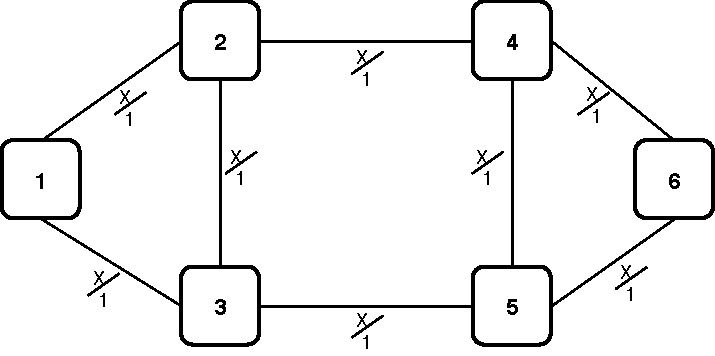
\includegraphics[width=11cm]{sdf/ilp/translucent_survivability/figures/allowed_physical_topology}
\caption{Allowed physical topology. The allowed physical topology is defined by the duct and sites in the field. It is assumed that each duct supports up to 1 bidirectional transmission system and each site supports up to 1 node.}
\label{allowed3_physical_low}
\end{figure}

\newpage
\begin{figure}[h!]
\centering
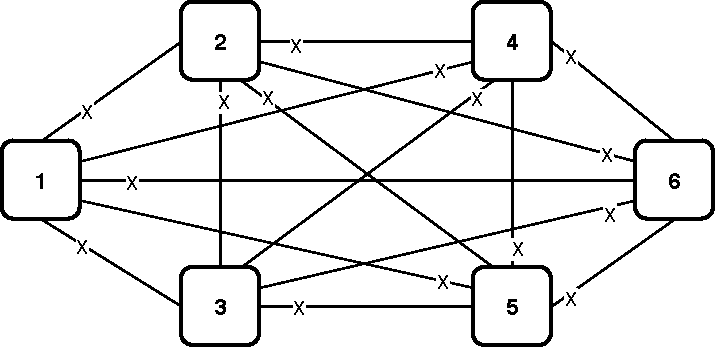
\includegraphics[width=11cm]{sdf/ilp/translucent_survivability/figures/allowed_optical_topology}
\caption{Allowed optical topology. The allowed optical topology is defined by the transport mode (translucent transport mode in this case). It is assumed that each connections between demands supports up to 100 lightpaths.}
\label{allowed3_optical_low}
\end{figure}

\begin{figure}[h!]
\centering
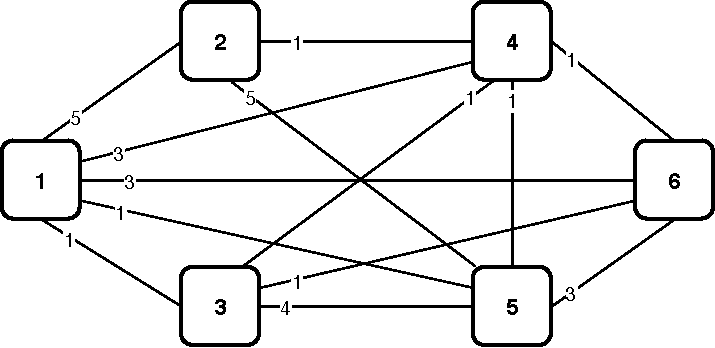
\includegraphics[width=11cm]{sdf/ilp/translucent_survivability/figures/logical_topology_ODU0_low}
\caption{ODU0 logical topology defined by the ODU0 traffic matrix.}
\label{logical3_ODU0_low}
\end{figure}

\begin{figure}[h!]
\centering
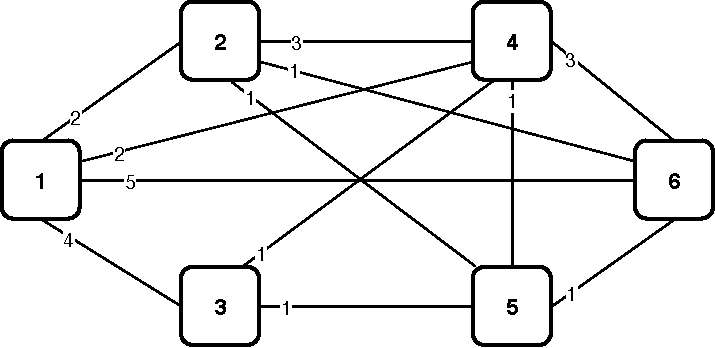
\includegraphics[width=11cm]{sdf/ilp/translucent_survivability/figures/logical_topology_ODU1_low}
\caption{ODU1 logical topology defined by the ODU1 traffic matrix.}
\label{logical3_ODU1_low}
\end{figure}

\newpage
\begin{figure}[h!]
\centering
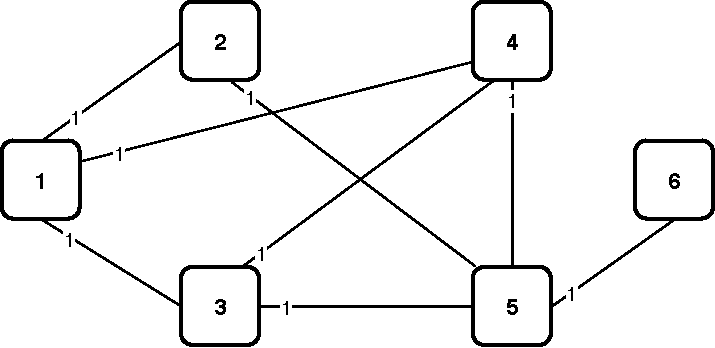
\includegraphics[width=12cm]{sdf/ilp/translucent_survivability/figures/logical_topology_ODU2_low}
\caption{ODU2 logical topology defined by the ODU2 traffic matrix.}
\label{logical3_ODU2_low}
\end{figure}

\begin{figure}[h!]
\centering
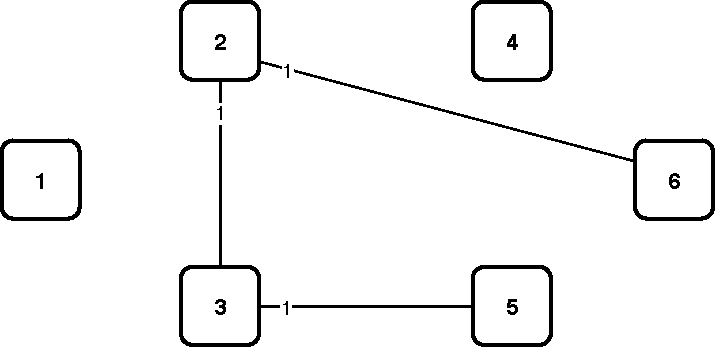
\includegraphics[width=12cm]{sdf/ilp/translucent_survivability/figures/logical_topology_ODU3_low}
\caption{ODU3 logical topology defined by the ODU3 traffic matrix.}
\label{logical3_ODU3_low}
\end{figure}

\begin{figure}[h!]
\centering
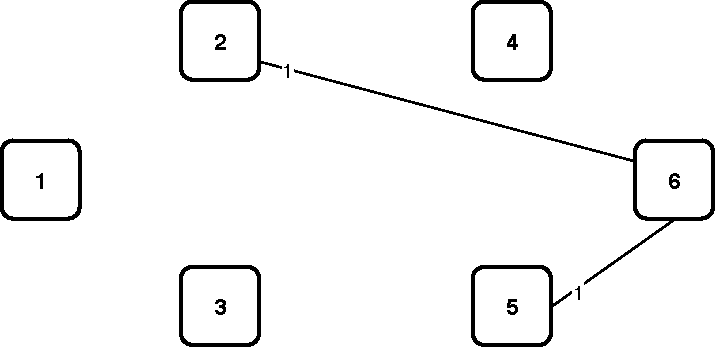
\includegraphics[width=12cm]{sdf/ilp/translucent_survivability/figures/logical_topology_ODU4_low}
\caption{ODU4 logical topology defined by the ODU4 traffic matrix.}
\label{logical3_ODU4_low}
\end{figure}
\newpage
\begin{figure}[h!]
\centering
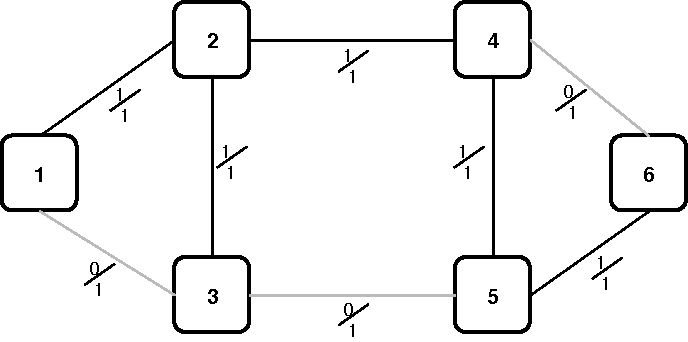
\includegraphics[width=12cm]{sdf/ilp/translucent_survivability/figures/physical_topology}
\caption{Physical topology after dimensioning.}
\label{physical3_low}
\end{figure}

\vspace{13pt}
\begin{figure}[h!]
\centering
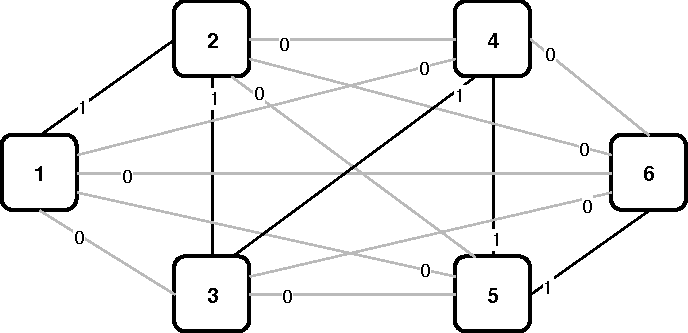
\includegraphics[width=12cm]{sdf/ilp/translucent_survivability/figures/optical_topology_low}
\caption{Optical topology after dimensioning.}
\label{optical3_low}
\end{figure}

\vspace{15pt}
In table \ref{link_transluc_surv_ref_low} we can see the number of optical channels calculated using \ref{Capex_Link} and \ref{ILPOpaque_CAPEX} and the number of amplifiers for each link calculated using \ref{Capex_amplifiers}. In the case where there are no optical channels we assume that the number of amplifiers is zero.\\

In table \ref{node_transluc_surv_ref_low} we can see the resulting nodal degree at the physical layer, calculated based on the number of connections that the node in question performs, the number of line ports and add ports using \ref{OXC_poxc_transluc} the number of long-reach transponders using \ref{EXC_pexc2_transluc} and the number of tributary ports using \ref{EXC_pexc1_transluc}.\\

\newpage
\begin{table}[h!]
\centering
\begin{tabular}{|| c | c | c ||}
 \hline
 \multicolumn{3}{|| c ||}{Information regarding links} \\
 \hline
 \hline
 Bidirectional Link & Optical Channels & Amplifiers\\
 \hline
 Node 1 <-> Node 2 & 1 & 4 \\
 Node 1 <-> Node 3 & 0 & 0 \\
 Node 2 <-> Node 3 & 2 & 0 \\
 Node 2 <-> Node 4 & 1 & 6 \\
 Node 3 <-> Node 5 & 0 & 0 \\
 Node 4 <-> Node 5 & 1 & 1 \\
 Node 4 <-> Node 6 & 0 & 0 \\
 Node 5 <-> Node 6 & 1 & 3 \\
 \hline
\end{tabular}
\caption{Table with information regarding links for translucent mode without survivability.}
\label{link_transluc_surv_ref_low}
\end{table}

\vspace{17pt}
\begin{table}[h!]
\centering
\begin{tabular}{|| c | c | c | c | c | c ||}
 \hline
 \multicolumn{6}{|| c ||}{Information regarding nodes} \\
 \hline
 \hline
 \multicolumn{2}{|| c |}{ } & \multicolumn{2}{ c |}{Electrical part} & \multicolumn{2}{ c ||}{Optical part} \\
 \hline
 Node & Resulting Nodal Degree & Tributary Ports & LR Transponders & Add Ports & Line Ports\\
 \hline
 1 & 1 & 29 & 1 & 1 & 1 \\
 2 & 3 & 23 & 2 & 2 & 4 \\
 3 & 1 & 18 & 2 & 2 & 2 \\
 4 & 2 & 20 & 2 & 2 & 2 \\
 5 & 2 & 24 & 2 & 2 & 2 \\
 6 & 1 & 22 & 1 & 1 & 1 \\
\hline
\end{tabular}
\caption{Table with information regarding nodes for translucent mode without survivability.}
\label{node_transluc_surv_ref_low}
\end{table}

\vspace{17pt}
Through the information obtained previously on the nodes we can now create tables with detailed information about each node. In each table mentioned below we can see how many ports are connected to a given node and its bit rate (in relation to the line ports) and how many ports are assigned to each different bit rate (in relation to the tributary ports).\\
\newpage
\begin{table}[h!]
\centering
\begin{tabular}{|| c | c | c ||}
 \hline
 \multicolumn{3}{|| c ||}{Detailed description of Node 1} \\
 \hline
 \hline
 Electrical part & Number of total demands & Bit rate \\
 \hline
\multirow{3}{*}{29 tributary ports} & 13 & ODU0 \\
 & 13 & ODU1 \\
 & 3 & ODU2 \\
 \hline
  & Node<--Optical Channels-->Node & Bit rate \\
 \hline
 1 LR Transponders & 1  <---- 1 ---->  2 & 100 Gbits/s \\
 \hline
 \hline
 Optical part & Node<--Optical Channels-->Node & Bit rate \\
 \hline
 1 add ports & 1  <---- 1 ---->  2 & 100 Gbits/s \\ \cline{1-2}
 1 line ports & 1  <---- 1 ---->  2 & \\
\hline
\end{tabular}
\caption{Table with detailed description of node 1. The number of demands is distributed to the various destination nodes, this distribution can be observed in section \ref{low_scenario}.}
\end{table}

\vspace{13pt}
\begin{table}[h!]
\centering
\begin{tabular}{|| c | c | c ||}
 \hline
 \multicolumn{3}{|| c ||}{Detailed description of Node 2} \\
 \hline
 \hline
 Electrical part & Number of total demands & Bit rate \\ \hline
\multirow{5}{*}{23 tributary ports} & 11 & ODU0 \\
 & 7 & ODU1 \\
 & 2 & ODU2 \\
 & 2 & ODU3 \\
 & 1 & ODU4 \\
 \hline
  & Node<--Optical Channels-->Node & Bit rate \\
  \hline
\multirow{2}{*}{2 LR Transponders} & 2  <---- 1 ---->  1 & \multirow{2}{*}{100 Gbits/s} \\
  & 2  <---- 1 ---->  3 & \\
 \hline
 \hline
 Optical part & Node<--Optical Channels-->Node & Bit rate \\
 \hline
 \multirow{2}{*}{2 add ports} & 2  <---- 1 ---->  1 & \multirow{5}{*}{100 Gbits/s} \\
  & 2  <---- 1 ---->  3 & \\ \cline{1-2}
 \multirow{3}{*}{4 line ports} & 2  <---- 1 ---->  1 & \\
  & 2  <---- 1 ---->  3 & \\
  & 3  <---- 1 ---->  4 & \\
\hline
\end{tabular}
\caption{Table with detailed description of node 2. The number of demands is distributed to the various destination nodes, this distribution can be observed in section \ref{low_scenario}. Regarding the number of line ports when this node is equal to the source, it means that add ports are used, otherwise it means that through ports are used. In the latter the number of ports is double the number of optical channels.}
\end{table}

\newpage
\begin{table}[h!]
\centering
\begin{tabular}{|| c | c | c ||}
 \hline
 \multicolumn{3}{|| c ||}{Detailed description of Node 3} \\
 \hline
 \hline
 Electrical part & Number of total demands & Bit rate \\
 \hline
 \multirow{4}{*}{18 tributary ports} & 7 & ODU0 \\
 & 6 & ODU1\\
 & 3 & ODU2\\
 & 2 & ODU3\\
 \hline
  & Node<--Optical Channels-->Node & Bit rate \\ \hline
 \multirow{2}{*}{2 LR Transponders} & 3  <---- 1 ---->  2 & \multirow{2}{*}{100 Gbits/s} \\
  & 3  <---- 1 ---->  4 & \\
 \hline
 \hline
 Optical part & Node<--Optical Channels-->Node & Bit rate \\
 \hline
 \multirow{2}{*}{2 add ports} & 3  <---- 1 ---->  2 & \multirow{4}{*}{100 Gbits/s} \\
  & 3  <---- 1 ---->  4 & \\ \cline{1-2}
 \multirow{2}{*}{2 line ports} & 3  <---- 1 ---->  2 & \\
  & 3  <---- 1 ---->  4 & \\
\hline
\end{tabular}
\caption{Table with detailed description of node 3. The number of demands is distributed to the various destination nodes, this distribution can be observed in section \ref{low_scenario}.}
\end{table}

\vspace{13pt}
\begin{table}[h!]
\centering
\begin{tabular}{|| c | c | c ||}
 \hline
 \multicolumn{3}{|| c ||}{Detailed description of Node 4} \\
 \hline
 \hline
 Electrical part & Number of total demands & Bit rate \\ \hline
\multirow{3}{*}{20 tributary ports} & 7 & ODU0 \\
 & 10 & ODU1 \\
 & 3 & ODU2 \\
 \hline
  & Node<--Optical Channels-->Node & Bit rate \\ \hline
 \multirow{2}{*}{2 LR Transponders} & 4  <---- 1 ---->  3 & \multirow{2}{*}{100 Gbits/s} \\
  & 4  <---- 1 ---->  5 & \\
 \hline
 \hline
 Optical part & Node<--Optical Channels-->Node & Bit rate \\
 \hline
 \multirow{2}{*}{2 add ports} & 4  <---- 1 ---->  3 & \multirow{4}{*}{100 Gbits/s} \\
  & 4  <---- 1 ---->  5 & \\ \cline{1-2}
 \multirow{2}{*}{2 line ports} & 4  <---- 1 ---->  3 & \\
  & 4  <---- 1 ---->  5 & \\
\hline
\end{tabular}
\caption{Table with detailed description of node 4. The number of demands is distributed to the various destination nodes, this distribution can be observed in section \ref{low_scenario}.}
\end{table}

\newpage
\begin{table}[h!]
\centering
\begin{tabular}{|| c | c | c ||}
 \hline
 \multicolumn{3}{|| c ||}{Detailed description of Node 5} \\
 \hline
 \hline
 Electrical part & Number of total demands & Bit rate \\ \hline
\multirow{5}{*}{24 tributary ports} & 14 & ODU0 \\
 & 4 & ODU1 \\
 & 4 & ODU2 \\
 & 1 & ODU3 \\
 & 1 & ODU4 \\
 \hline
  & Node<--Optical Channels-->Node & Bit rate \\ \hline
 \multirow{2}{*}{2 LR Transponders} & 5  <---- 1 ---->  4 & \multirow{2}{*}{100 Gbits/s} \\
  & 5  <---- 2 ---->  6 & \\
 \hline
 \hline
 Optical part & Node<--Optical Channels-->Node & Bit rate \\
 \hline
 \multirow{2}{*}{2 add ports} & 5  <---- 1 ---->  4 & \multirow{4}{*}{100 Gbits/s} \\
  & 5  <---- 2 ---->  6 & \\ \cline{1-2}
 \multirow{2}{*}{2 line ports} & 5  <---- 1 ---->  4 & \\
  & 5  <---- 2 ---->  6 & \\
\hline
\end{tabular}
\caption{Table with detailed description of node 5. The number of demands is distributed to the various destination nodes, this distribution can be observed in section \ref{low_scenario}.}
\end{table}

\vspace{13pt}
\begin{table}[h!]
\centering
\begin{tabular}{|| c | c | c ||}
 \hline
 \multicolumn{3}{|| c ||}{Detailed description of Node 6} \\
 \hline
 \hline
 Electrical part & Number of total demands & Bit rate \\ \hline
\multirow{5}{*}{22 tributary ports} & 8 & ODU0 \\
 & 10 & ODU1 \\
 & 1 & ODU2 \\
 & 1 & ODU3 \\
 & 2 & ODU4 \\
 \hline
  & Node<--Optical Channels-->Node & Bit rate \\ \hline
 1 LR Transponders & 6  <---- 1 ---->  5 & 100 Gbits/s \\
 \hline
 Optical part & Node<--Optical Channels-->Node & Bit rate \\
 \hline
 1 add ports & 6  <---- 1 ---->  5 & 100 Gbits/s \\ \cline{1-2}
 1 line ports & 6  <---- 1 ---->  5 & \\
\hline
\end{tabular}
\caption{Table with detailed description of node 6. The number of demands is distributed to the various destination nodes, this distribution can be observed in section \ref{low_scenario}.}
\end{table}

\vspace{17pt}
Now, in next page, let's focus on the routing information in table \ref{path_transluc_surv_ref_low}. These paths are bidirectional so the path from one node to another is the same path in the opposite direction.\\

\begin{table}[h!]
\centering
\begin{tabular}{|| c | c | c ||}
 \hline
 \multicolumn{3}{|| c ||}{Routing} \\
 \hline
 \hline
 o & d & Links \\
 \hline
 1 & 2 & \{(1,2)\} \\ \hline
 1 & 3 & \{(1,2),(2,3)\} \\ \hline
 1 & 4 & \{(1,2),(2,4)\}\\ \hline
 1 & 5 & \{(1,2),(2,4),(4,5)\}\\ \hline
 1 & 6 & \{(1,2),(2,4),(4,5),(5,6)\}\\ \hline
 2 & 3 & \{(2,3)\}\\ \hline
 2 & 4 & \{(2,4)\}\\ \hline
 2 & 5 & \{(2,4),(4,5)\}\\ \hline
 2 & 6 & \{(2,4),(4,5),(5,6)\}\\ \hline
 3 & 4 & \{(3,2),(2,4)\}\\ \hline
 3 & 5 & \{(3,2),(2,4),(4,5)\}\\ \hline
 3 & 6 & \{(3,2),(2,4),(4,5),(5,6)\}\\ \hline
 4 & 5 & \{(4,5)\}\\ \hline
 4 & 6 & \{(4,5),(5,6)\}\\ \hline
 5 & 6 & \{(5,6)\}\\
 \hline
\end{tabular}
\caption{Table with description of routing.}
\label{path_transluc_surv_ref_low}
\end{table}

Finally and most importantly through table \ref{scripttransluc_surv_ref_low} we can see the CAPEX result for this model. This value is obtained using equation \ref{ILPOpaque_CAPEX} and all of the constraints mentioned above.\\

\begin{table}[h!]
\centering
\begin{tabular}{|| c | c | c | c | c | c | c ||}
 \hline
 \multicolumn{7}{|| c ||}{CAPEX of the Network} \\
 \hline
 \hline
 \multicolumn{3}{|| c |}{ } & Quantity & Unit Price & Cost & Total \\
 \hline
 \multirow{3}{*}{Link Cost} & \multicolumn{2}{ c |}{OLTs} & 10 & 15 000 \euro & 150 000 \euro & \multirow{3}{*}{6 262 000 \euro} \\ \cline{2-6}
 & \multicolumn{2}{ c |}{100 Gbits/s Transceivers} & 12 & 5 000 \euro/Gbit/s & 6 000 000 \euro & \\ \cline{2-6}
 & \multicolumn{2}{ c |}{Amplifiers} & 28 & 4 000 \euro & 112 000 \euro & \\
 \hline
 \multirow{10}{*}{Node Cost} & \multirow{7}{*}{Electrical} & EXCs & 6 & 10 000 \euro & 60 000 \euro & \multirow{10}{*}{1 237 590 \euro} \\ \cline{3-6}
 & & ODU0 Ports & 60 & 10 \euro/port & 600 \euro & \\ \cline{3-6}
 & & ODU1 Ports & 50 & 15 \euro/port & 750 \euro & \\ \cline{3-6}
 & & ODU2 Ports & 16 & 30 \euro/port & 480 \euro & \\ \cline{3-6}
 & & ODU3 Ports & 6 & 60 \euro/port & 360 \euro & \\ \cline{3-6}
 & & ODU4 Ports & 4 & 100 \euro/port & 400 \euro & \\ \cline{3-6}
 & &Transponders& 10 & 100 000 \euro/port & 1 000 000 \euro & \\ \cline{2-6}
 & \multirow{3}{*}{Optical} & OXCs & 6 & 20 000 \euro & 120 000 \euro & \\ \cline{3-6}
 & & Line Ports & 12 & 2 500 \euro/port & 30 000 \euro & \\ \cline{3-6}
 & & Add Ports & 10 & 2 500 \euro/port & 25 000 \euro & \\
 \hline
 \multicolumn{6}{|| c |}{Total Network Cost} & 7 499 590 \euro \\
\hline
\end{tabular}
\caption{Table with detailed description of CAPEX for this scenario.}
\label{scripttransluc_surv_ref_low}
\end{table}

\newpage
\textbf{Medium Traffic Scenario:}\\

In this scenario we have to take into account the traffic calculated in \ref{medium_traffic_scenario}. In a first phase we will show the various existing topologies of the network. The first are the allowed topologies, physical and optical topology, the second are the logical topology for all ODUs and finally the resulting physical and optical topology.\\

\begin{figure}[h!]
\centering
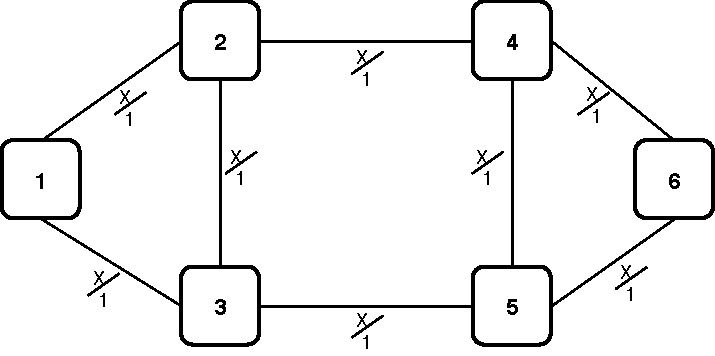
\includegraphics[width=12cm]{sdf/ilp/translucent_survivability/figures/allowed_physical_topology}
\caption{Allowed physical topology. The allowed physical topology is defined by the duct and sites in the field. It is assumed that each duct supports up to 1 bidirectional transmission system and each site supports up to 1 node.}
\label{allowed3_physical_medium}
\end{figure}
\vspace{11pt}
\begin{figure}[h!]
\centering
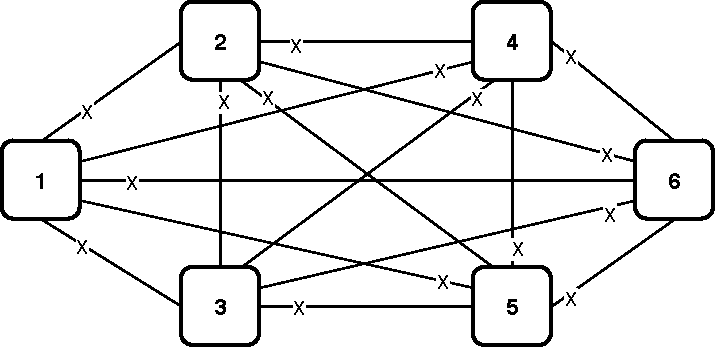
\includegraphics[width=12cm]{sdf/ilp/translucent_survivability/figures/allowed_optical_topology}
\caption{Allowed optical topology. The allowed optical topology is defined by the transport mode (translucent transport mode in this case). It is assumed that each connections between demands supports up to 100 lightpaths.}
\label{allowed3_optical_medium}
\end{figure}

\newpage
\begin{figure}[h!]
\centering
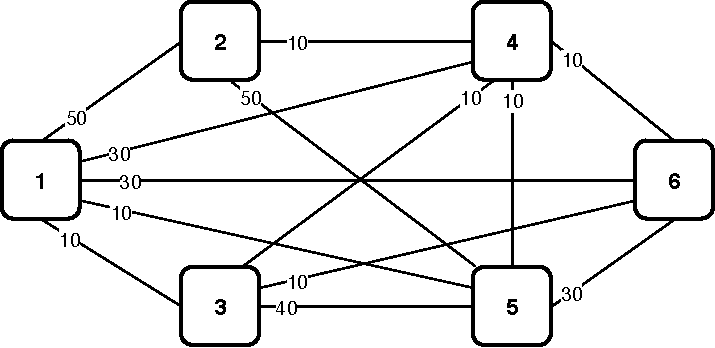
\includegraphics[width=12cm]{sdf/ilp/translucent_survivability/figures/logical_topology_ODU0_medium}
\caption{ODU0 logical topology defined by the ODU0 traffic matrix.}
\label{logical3_ODU0_medium}
\end{figure}

\begin{figure}[h!]
\centering
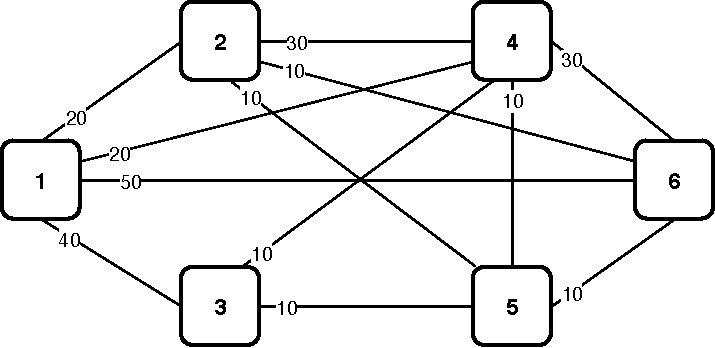
\includegraphics[width=12cm]{sdf/ilp/translucent_survivability/figures/logical_topology_ODU1_medium}
\caption{ODU1 logical topology defined by the ODU1 traffic matrix.}
\label{logical3_ODU1_medium}
\end{figure}

\begin{figure}[h!]
\centering
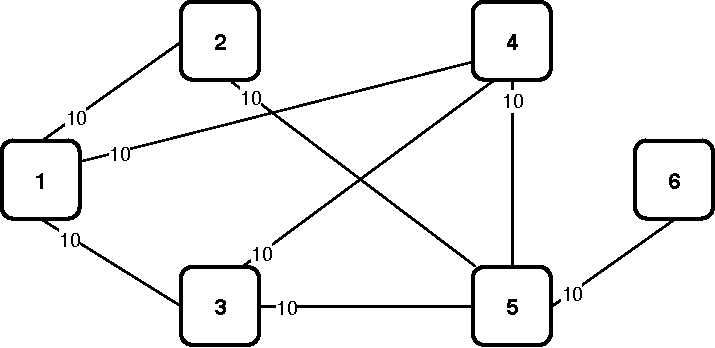
\includegraphics[width=12cm]{sdf/ilp/translucent_survivability/figures/logical_topology_ODU2_medium}
\caption{ODU2 logical topology defined by the ODU2 traffic matrix.}
\label{logical3_ODU2_medium}
\end{figure}

\begin{figure}[h!]
\centering
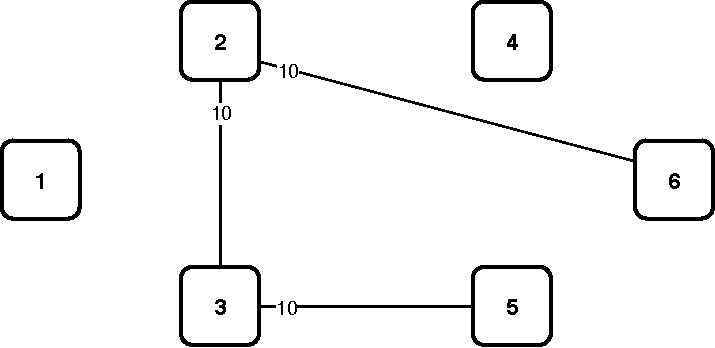
\includegraphics[width=12cm]{sdf/ilp/translucent_survivability/figures/logical_topology_ODU3_medium}
\caption{ODU3 logical topology defined by the ODU3 traffic matrix.}
\label{logical3_ODU3_medium}
\end{figure}

\begin{figure}[h!]
\centering
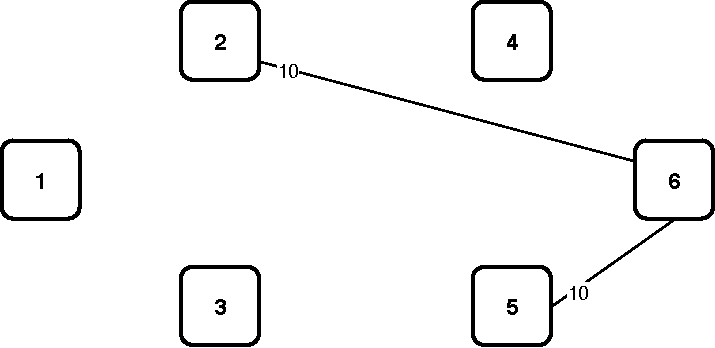
\includegraphics[width=12cm]{sdf/ilp/translucent_survivability/figures/logical_topology_ODU4_medium}
\caption{ODU4 logical topology defined by the ODU4 traffic matrix.}
\label{logical3_ODU4_medium}
\end{figure}

\begin{figure}[h!]
\centering
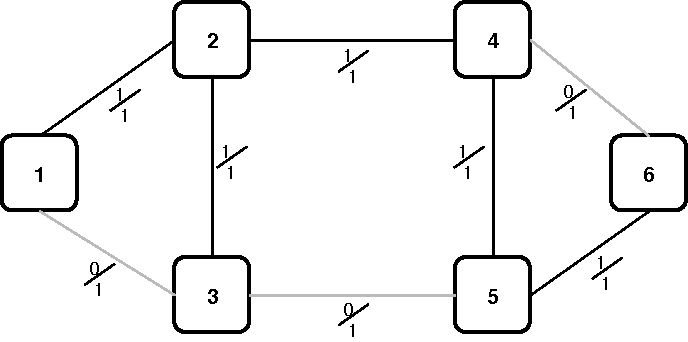
\includegraphics[width=12cm]{sdf/ilp/translucent_survivability/figures/physical_topology}
\caption{Physical topology after dimensioning.}
\label{physical3_medium}
\end{figure}

\newpage
\begin{figure}[h!]
\centering
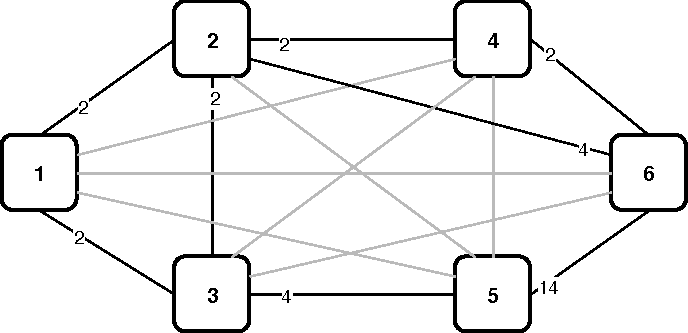
\includegraphics[width=13cm]{sdf/ilp/translucent_survivability/figures/optical_topology_medium}
\caption{Optical topology after dimensioning.}
\label{optical3_medium}
\end{figure}

\vspace{15pt}
In table \ref{link_transluc_surv_ref_medium} we can see the number of optical channels calculated using \ref{Capex_Link} and \ref{ILPOpaque_CAPEX} and the number of amplifiers for each link calculated using \ref{Capex_amplifiers}. In the case where there are no optical channels we assume that the number of amplifiers is zero.\\

\begin{table}[h!]
\centering
\begin{tabular}{|| c | c | c ||}
 \hline
 \multicolumn{3}{|| c ||}{Information regarding links} \\
 \hline
 \hline
 Bidirectional Link & Optical Channels & Amplifiers\\
 \hline
 Node 1 <-> Node 2 & 2 & 4 \\
 Node 1 <-> Node 3 & 0 & 0 \\
 Node 2 <-> Node 3 & 10 & 0 \\
 Node 2 <-> Node 4 & 2 & 6 \\
 Node 3 <-> Node 5 & 0 & 0 \\
 Node 4 <-> Node 5 & 1 & 1 \\
 Node 4 <-> Node 6 & 0 & 0 \\
 Node 5 <-> Node 6 & 5 & 3 \\
 \hline
\end{tabular}
\caption{Table with information regarding links for translucent mode without survivability.}
\label{link_transluc_surv_ref_medium}
\end{table}

\vspace{15pt}
In table \ref{node_transluc_surv_ref_medium} we can see the resulting nodal degree at the physical layer, calculated based on the number of connections that the node in question performs, the number of line ports and add ports using \ref{OXC_poxc_transluc} the number of long-reach transponders using \ref{EXC_pexc2_transluc} and the number of tributary ports using \ref{EXC_pexc1_transluc}.\\

\newpage

\begin{table}[h!]
\centering
\begin{tabular}{|| c | c | c | c | c | c ||}
 \hline
 \multicolumn{6}{|| c ||}{Information regarding nodes} \\
 \hline
 \hline
 \multicolumn{2}{|| c |}{ } & \multicolumn{2}{ c |}{Electrical part} & \multicolumn{2}{ c ||}{Optical part} \\
 \hline
 Node & Resulting Nodal Degree & Tributary Ports & LR Transponders & Add Ports & Line Ports\\
 \hline
 1 & 1 & 290 & 2 & 2 & 2 \\
 2 & 3 & 230 & 10 & 10 & 14 \\
 3 & 1 & 180 & 10 & 10 & 10 \\
 4 & 2 & 200 & 3 & 3 & 3 \\
 5 & 2 & 240 & 6 & 6 & 6 \\
 6 & 1 & 220 & 5 & 5 & 5 \\
\hline
\end{tabular}
\caption{Table with information regarding nodes for translucent mode without survivability.}
\label{node_transluc_surv_ref_medium}
\end{table}

\vspace{17pt}
Through the information obtained previously on the nodes we can now create tables with detailed information about each node. In each table mentioned below we can see how many ports are connected to a given node and its bit rate (in relation to the line ports) and how many ports are assigned to each different bit rate (in relation to the tributary ports).\\

\begin{table}[h!]
\centering
\begin{tabular}{|| c | c | c ||}
 \hline
 \multicolumn{3}{|| c ||}{Detailed description of Node 1} \\
 \hline
 \hline
 Electrical part & Number of total demands & Bit rate \\
 \hline
\multirow{3}{*}{290 tributary ports} & 130 & ODU0 \\
 & 130 & ODU1 \\
 & 30 & ODU2 \\
 \hline
  & Node<--Optical Channels-->Node & Bit rate \\
 \hline
 2 LR Transponders & 1  <---- 2 ---->  2 & 100 Gbits/s \\
 \hline
 \hline
 Optical part & Node<--Optical Channels-->Node & Bit rate \\
 \hline
 2 add ports & 1  <---- 2 ---->  2 & 100 Gbits/s \\ \cline{1-2}
 2 line ports & 1  <---- 2 ---->  2 & \\
\hline
\end{tabular}
\caption{Table with detailed description of node 1. The number of demands is distributed to the various destination nodes, this distribution can be observed in section \ref{medium_traffic_scenario}.}
\end{table}

\newpage
\begin{table}[h!]
\centering
\begin{tabular}{|| c | c | c ||}
 \hline
 \multicolumn{3}{|| c ||}{Detailed description of Node 2} \\
 \hline
 \hline
 Electrical part & Number of total demands & Bit rate \\ \hline
\multirow{5}{*}{230 tributary ports} & 110 & ODU0 \\
 & 70 & ODU1 \\
 & 20 & ODU2 \\
 & 20 & ODU3 \\
 & 10 & ODU4 \\
 \hline
  & Node<--Optical Channels-->Node & Bit rate \\
  \hline
\multirow{2}{*}{10 LR Transponders} & 2  <---- 2 ---->  1 & \multirow{2}{*}{100 Gbits/s} \\
  & 2  <---- 8 ---->  3 & \\
 \hline
 \hline
 Optical part & Node<--Optical Channels-->Node & Bit rate \\
 \hline
 \multirow{2}{*}{10 add ports} & 2  <---- 2 ---->  1 & \multirow{5}{*}{100 Gbits/s} \\
  & 2  <---- 8 ---->  3 & \\ \cline{1-2}
 \multirow{3}{*}{14 line ports} & 2  <---- 2 ---->  1 & \\
  & 2  <---- 8 ---->  3 & \\
  & 3  <---- 2 ---->  4 & \\
\hline
\end{tabular}
\caption{Table with detailed description of node 2. The number of demands is distributed to the various destination nodes, this distribution can be observed in section \ref{medium_traffic_scenario}. Regarding the number of line ports when this node is equal to the source, it means that add ports are used, otherwise it means that through ports are used.}
\end{table}

\begin{table}[h!]
\centering
\begin{tabular}{|| c | c | c ||}
 \hline
 \multicolumn{3}{|| c ||}{Detailed description of Node 3} \\
 \hline
 \hline
 Electrical part & Number of total demands & Bit rate \\
 \hline
 \multirow{4}{*}{180 tributary ports} & 70 & ODU0 \\
 & 60 & ODU1\\
 & 30 & ODU2\\
 & 20 & ODU3\\
 \hline
  & Node<--Optical Channels-->Node & Bit rate \\ \hline
 \multirow{2}{*}{10 LR Transponders} & 3  <---- 8 ---->  2 & \multirow{2}{*}{100 Gbits/s} \\
  & 3  <---- 2 ---->  4 & \\
 \hline
 \hline
 Optical part & Node<--Optical Channels-->Node & Bit rate \\
 \hline
 \multirow{2}{*}{10 add ports} & 3  <---- 8 ---->  2 & \multirow{4}{*}{100 Gbits/s} \\
  & 3  <---- 2 ---->  4 & \\ \cline{1-2}
 \multirow{2}{*}{10 line ports} & 3  <---- 8 ---->  2 & \\
  & 3  <---- 2 ---->  4 & \\
\hline
\end{tabular}
\caption{Table with detailed description of node 3. The number of demands is distributed to the various destination nodes, this distribution can be observed in section \ref{medium_traffic_scenario}.}
\end{table}

\newpage
\begin{table}[h!]
\centering
\begin{tabular}{|| c | c | c ||}
 \hline
 \multicolumn{3}{|| c ||}{Detailed description of Node 4} \\
 \hline
 \hline
 Electrical part & Number of total demands & Bit rate \\ \hline
\multirow{3}{*}{200 tributary ports} & 70 & ODU0 \\
 & 100 & ODU1 \\
 & 30 & ODU2 \\
 \hline
  & Node<--Optical Channels-->Node & Bit rate \\ \hline
 \multirow{2}{*}{3 LR Transponders} & 4  <---- 2 ---->  3 & \multirow{2}{*}{100 Gbits/s} \\
  & 4  <---- 1 ---->  5 & \\
 \hline
 \hline
 Optical part & Node<--Optical Channels-->Node & Bit rate \\
 \hline
 \multirow{2}{*}{3 add ports} & 4  <---- 2 ---->  3 & \multirow{4}{*}{100 Gbits/s} \\
  & 4  <---- 1 ---->  5 & \\ \cline{1-2}
 \multirow{2}{*}{3 line ports} & 4  <---- 2 ---->  3 & \\
  & 4  <---- 1 ---->  5 & \\
\hline
\end{tabular}
\caption{Table with detailed description of node 4. The number of demands is distributed to the various destination nodes, this distribution can be observed in section \ref{medium_traffic_scenario}.}
\end{table}

\vspace{13pt}
\begin{table}[h!]
\centering
\begin{tabular}{|| c | c | c ||}
 \hline
 \multicolumn{3}{|| c ||}{Detailed description of Node 5} \\
 \hline
 \hline
 Electrical part & Number of total demands & Bit rate \\ \hline
\multirow{5}{*}{240 tributary ports} & 140 & ODU0 \\
 & 40 & ODU1 \\
 & 40 & ODU2 \\
 & 10 & ODU3 \\
 & 10 & ODU4 \\
 \hline
  & Node<--Optical Channels-->Node & Bit rate \\ \hline
 \multirow{2}{*}{6 LR Transponders} & 5  <---- 1 ---->  4 & \multirow{2}{*}{100 Gbits/s} \\
  & 5  <---- 5 ---->  6 & \\
 \hline
 \hline
 Optical part & Node<--Optical Channels-->Node & Bit rate \\
 \hline
 \multirow{2}{*}{6 add ports} & 5  <---- 1 ---->  4 & \multirow{4}{*}{100 Gbits/s} \\
  & 5  <---- 5 ---->  6 & \\ \cline{1-2}
 \multirow{2}{*}{6 line ports} & 5  <---- 1 ---->  4 & \\
  & 5  <---- 5 ---->  6 & \\
\hline
\end{tabular}
\caption{Table with detailed description of node 5. The number of demands is distributed to the various destination nodes, this distribution can be observed in section \ref{medium_traffic_scenario}.}
\end{table}

\newpage
\begin{table}[h!]
\centering
\begin{tabular}{|| c | c | c ||}
 \hline
 \multicolumn{3}{|| c ||}{Detailed description of Node 6} \\
 \hline
 \hline
 Electrical part & Number of total demands & Bit rate \\ \hline
\multirow{5}{*}{220 tributary ports} & 80 & ODU0 \\
 & 100 & ODU1 \\
 & 10 & ODU2 \\
 & 10 & ODU3 \\
 & 20 & ODU4 \\
 \hline
  & Node<--Optical Channels-->Node & Bit rate \\ \hline
 5 LR Transponders & 6  <---- 5 ---->  5 & 100 Gbits/s \\
 \hline
 Optical part & Node<--Optical Channels-->Node & Bit rate \\
 \hline
 5 add ports & 6  <---- 5 ---->  5 & 100 Gbits/s \\ \cline{1-2}
 5 line ports & 6  <---- 5 ---->  5 & \\
\hline
\end{tabular}
\caption{Table with detailed description of node 6. The number of demands is distributed to the various destination nodes, this distribution can be observed in section \ref{medium_traffic_scenario}.}
\end{table}

Now let's focus on the routing information in table \ref{path_transluc_surv_ref_low}. These paths are bidirectional so the path from one node to another is the same path in the opposite direction.\\

\begin{table}[h!]
\centering
\begin{tabular}{|| c | c | c ||}
 \hline
 \multicolumn{3}{|| c ||}{Routing} \\
 \hline
 \hline
 o & d & Links \\
 \hline
 1 & 2 & \{(1,2)\} \\ \hline
 1 & 3 & \{(1,2),(2,3)\} \\ \hline
 1 & 4 & \{(1,2),(2,4)\}\\ \hline
 1 & 5 & \{(1,2),(2,4),(4,5)\}\\ \hline
 1 & 6 & \{(1,2),(2,4),(4,5),(5,6)\}\\ \hline
 2 & 3 & \{(2,3)\}\\ \hline
 2 & 4 & \{(2,4)\}\\ \hline
 2 & 5 & \{(2,4),(4,5)\}\\ \hline
 2 & 6 & \{(2,4),(4,5),(5,6)\}\\ \hline
 3 & 4 & \{(3,2),(2,4)\}\\ \hline
 3 & 5 & \{(3,2),(2,4),(4,5)\}\\ \hline
 3 & 6 & \{(3,2),(2,4),(4,5),(5,6)\}\\ \hline
 4 & 5 & \{(4,5)\}\\ \hline
 4 & 6 & \{(4,5),(5,6)\}\\ \hline
 5 & 6 & \{(5,6)\}\\
 \hline
\end{tabular}
\caption{Table with description of routing.}
\label{path_transluc_surv_ref_medium}
\end{table}

Finally and most importantly through table \ref{scripttransluc_surv_ref_medium} we can see the CAPEX result for this model. This value is obtained using equation \ref{ILPOpaque_CAPEX} and all of the constraints mentioned above.\\

\begin{table}[h!]
\centering
\begin{tabular}{|| c | c | c | c | c | c | c ||}
 \hline
 \multicolumn{7}{|| c ||}{CAPEX of the Network} \\
 \hline
 \hline
 \multicolumn{3}{|| c |}{ } & Quantity & Unit Price & Cost & Total \\
 \hline
 \multirow{3}{*}{Link Cost} & \multicolumn{2}{ c |}{OLTs} & 10 & 15 000 \euro & 150 000 \euro & \multirow{3}{*}{20 262 000 \euro} \\ \cline{2-6}
 & \multicolumn{2}{ c |}{100 Gbits/s Transceivers} & 40 & 5 000 \euro/Gbit/s & 20 000 000 \euro & \\ \cline{2-6}
 & \multicolumn{2}{ c |}{Amplifiers} & 28 & 4 000 \euro & 112 000 \euro & \\
 \hline
 \multirow{10}{*}{Node Cost} & \multirow{7}{*}{Electrical} & EXCs & 6 & 10 000 \euro & 60 000 \euro & \multirow{10}{*}{3 995 900 \euro} \\ \cline{3-6}
 & & ODU0 Ports & 600 & 10 \euro/port & 6 000 \euro & \\ \cline{3-6}
 & & ODU1 Ports & 500 & 15 \euro/port & 7 500 \euro & \\ \cline{3-6}
 & & ODU2 Ports & 160 & 30 \euro/port & 4 800 \euro & \\ \cline{3-6}
 & & ODU3 Ports & 60 & 60 \euro/port & 3 600 \euro & \\ \cline{3-6}
 & & ODU4 Ports & 40 & 100 \euro/port & 4 000 \euro & \\ \cline{3-6}
 & &Transponders& 36 & 100 000 \euro/port & 3 600 000 \euro & \\ \cline{2-6}
 & \multirow{3}{*}{Optical} & OXCs & 6 & 20 000 \euro & 120 000 \euro & \\ \cline{3-6}
 & & Line Ports & 40 & 2 500 \euro/port & 100 000 \euro & \\ \cline{3-6}
 & & Add Ports & 36 & 2 500 \euro/port & 90 000 \euro & \\
 \hline
 \multicolumn{6}{|| c |}{Total Network Cost} & 24 257 900 \euro \\
\hline
\end{tabular}
\caption{Table with detailed description of CAPEX for this scenario.}
\label{scripttransluc_surv_ref_medium}
\end{table}

\vspace{13pt}
\textbf{High Traffic Scenario:}\\

In this scenario we have to take into account the traffic calculated in \ref{high_traffic_scenario}. In a first phase we will show the various existing topologies of the network. The first are the allowed topologies, physical and optical topology, the second are the logical topology for all ODUs and finally the resulting physical and optical topology.

\begin{figure}[h!]
\centering
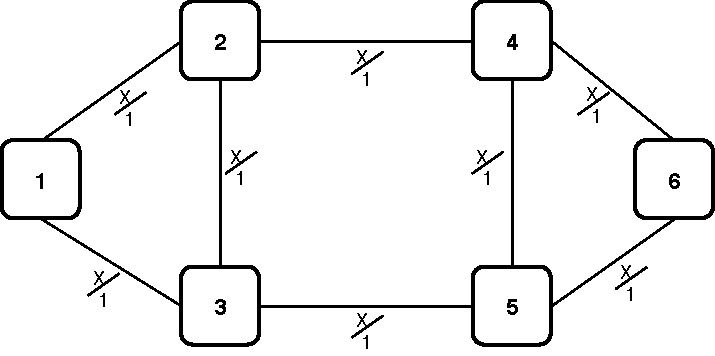
\includegraphics[width=11cm]{sdf/ilp/translucent_survivability/figures/allowed_physical_topology}
\caption{Allowed physical topology. The allowed physical topology is defined by the duct and sites in the field. It is assumed that each duct supports up to 1 bidirectional transmission system and each site supports up to 1 node.}
\label{allowed3_physical_high}
\end{figure}

\newpage
\begin{figure}[h!]
\centering
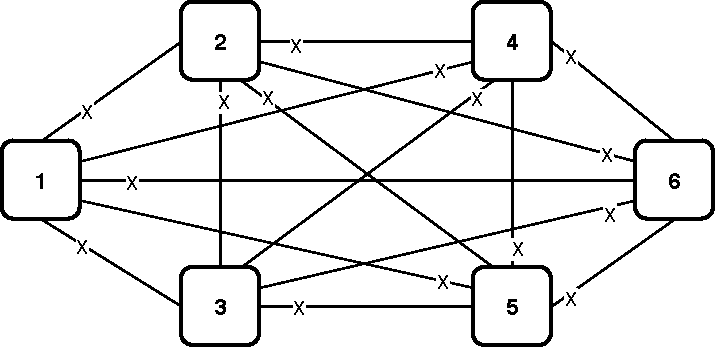
\includegraphics[width=11cm]{sdf/ilp/translucent_survivability/figures/allowed_optical_topology}
\caption{Allowed optical topology. The allowed optical topology is defined by the transport mode (translucent transport mode in this case). It is assumed that each connections between demands supports up to 100 lightpaths.}
\label{allowed3_optical_high}
\end{figure}

\begin{figure}[h!]
\centering
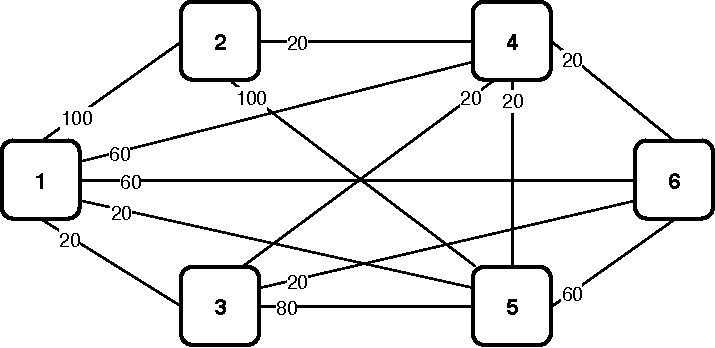
\includegraphics[width=11cm]{sdf/ilp/translucent_survivability/figures/logical_topology_ODU0_high}
\caption{ODU0 logical topology defined by the ODU0 traffic matrix.}
\label{logical3_ODU0_high}
\end{figure}

\begin{figure}[h!]
\centering
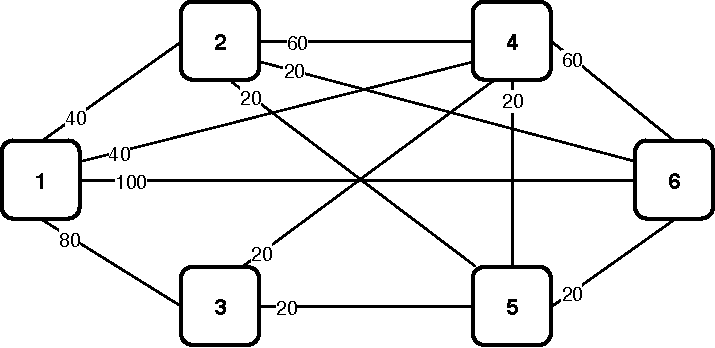
\includegraphics[width=11cm]{sdf/ilp/translucent_survivability/figures/logical_topology_ODU1_high}
\caption{ODU1 logical topology defined by the ODU1 traffic matrix.}
\label{logical3_ODU1_high}
\end{figure}
\newpage
\begin{figure}[h!]
\centering
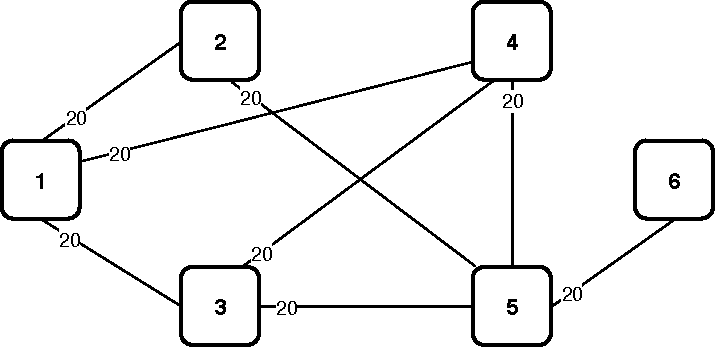
\includegraphics[width=12cm]{sdf/ilp/translucent_survivability/figures/logical_topology_ODU2_high}
\caption{ODU2 logical topology defined by the ODU2 traffic matrix.}
\label{logical3_ODU2_high}
\end{figure}

\begin{figure}[h!]
\centering
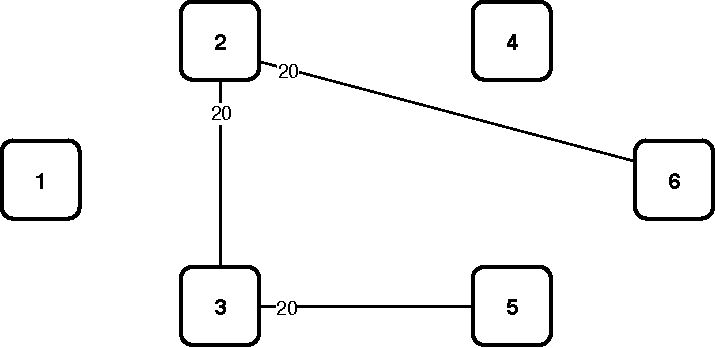
\includegraphics[width=12cm]{sdf/ilp/translucent_survivability/figures/logical_topology_ODU3_high}
\caption{ODU3 logical topology defined by the ODU3 traffic matrix.}
\label{logical3_ODU3_high}
\end{figure}

\begin{figure}[h!]
\centering
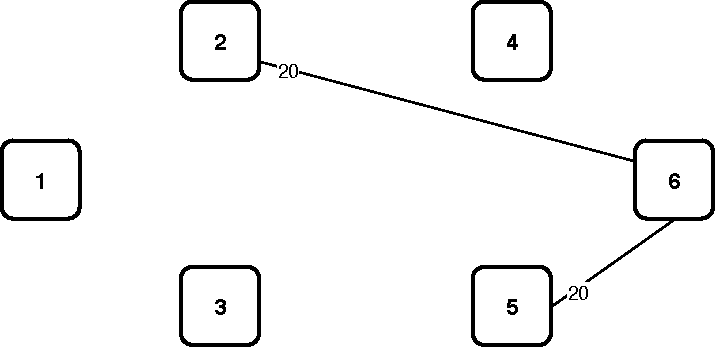
\includegraphics[width=12cm]{sdf/ilp/translucent_survivability/figures/logical_topology_ODU4_high}
\caption{ODU4 logical topology defined by the ODU4 traffic matrix.}
\label{logical3_ODU4_high}
\end{figure}
\newpage
\begin{figure}[h!]
\centering
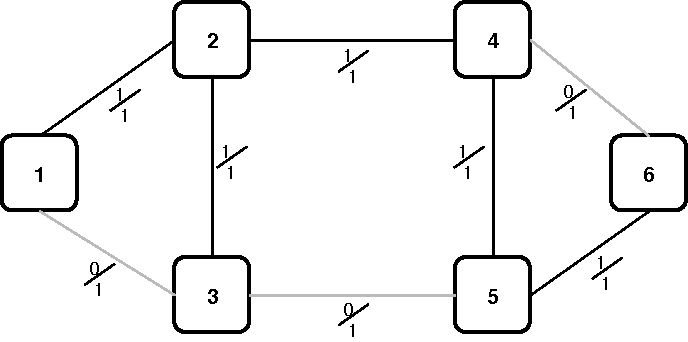
\includegraphics[width=13cm]{sdf/ilp/translucent_survivability/figures/physical_topology}
\caption{Physical topology after dimensioning.}
\label{physical3_high}
\end{figure}

\vspace{13pt}
\begin{figure}[h!]
\centering
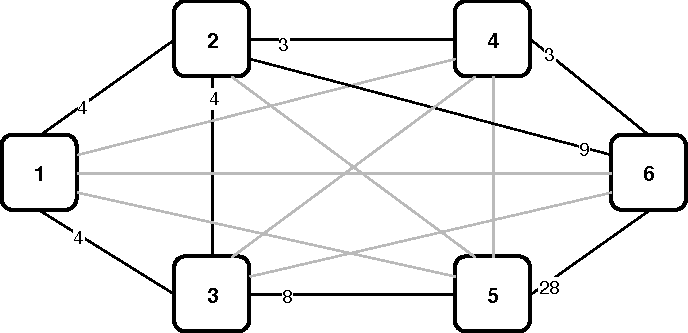
\includegraphics[width=13cm]{sdf/ilp/translucent_survivability/figures/optical_topology_high}
\caption{Optical topology after dimensioning.}
\label{optical3_high}
\end{figure}

\vspace{15pt}
In table \ref{link_transluc_surv_ref_high} we can see the number of optical channels calculated using \ref{Capex_Link} and \ref{ILPOpaque_CAPEX} and the number of amplifiers for each link calculated using \ref{Capex_amplifiers}. In the case where there are no optical channels we assume that the number of amplifiers is zero.\\

In table \ref{node_transluc_surv_ref_high} we can see the resulting nodal degree at the physical layer, calculated based on the number of connections that the node in question performs, the number of line ports and add ports using \ref{OXC_poxc_transluc} the number of long-reach transponders using \ref{EXC_pexc2_transluc} and the number of tributary ports using \ref{EXC_pexc1_transluc}.\\
\newpage
\begin{table}[h!]
\centering
\begin{tabular}{|| c | c | c ||}
 \hline
 \multicolumn{3}{|| c ||}{Information regarding links} \\
 \hline
 \hline
 Bidirectional Link & Optical Channels & Amplifiers\\
 \hline
 Node 1 <-> Node 2 & 4 & 4 \\
 Node 1 <-> Node 3 & 0 & 0 \\
 Node 2 <-> Node 3 & 20 & 0 \\
 Node 2 <-> Node 4 & 4 & 6 \\
 Node 3 <-> Node 5 & 0 & 0 \\
 Node 4 <-> Node 5 & 1 & 1 \\
 Node 4 <-> Node 6 & 0 & 0 \\
 Node 5 <-> Node 6 & 10 & 3 \\
 \hline
\end{tabular}
\caption{Table with information regarding links for translucent mode without survivability.}
\label{link_transluc_surv_ref_high}
\end{table}

\vspace{17pt}
\begin{table}[h!]
\centering
\begin{tabular}{|| c | c | c | c | c | c ||}
 \hline
 \multicolumn{6}{|| c ||}{Information regarding nodes} \\
 \hline
 \hline
 \multicolumn{2}{|| c |}{ } & \multicolumn{2}{ c |}{Electrical part} & \multicolumn{2}{ c ||}{Optical part} \\
 \hline
 Node & Resulting Nodal Degree & Tributary Ports & LR Transponders & Add Ports & Line Ports\\
 \hline
 1 & 1 & 580 & 4 & 4 & 4 \\
 2 & 3 & 460 & 20 & 20 & 28 \\
 3 & 1 & 360 & 20 & 20 & 20 \\
 4 & 2 & 400 & 5 & 5 & 5 \\
 5 & 2 & 480 & 11 & 11 & 11 \\
 6 & 1 & 440 & 10 & 10 & 10 \\
\hline
\end{tabular}
\caption{Table with information regarding nodes for translucent mode without survivability.}
\label{node_transluc_surv_ref_high}
\end{table}

\vspace{17pt}
Through the information obtained previously on the nodes we can now create tables with detailed information about each node. In each table mentioned below we can see how many ports are connected to a given node and its bit rate (in relation to the line ports) and how many ports are assigned to each different bit rate (in relation to the tributary ports).\\
\newpage
\begin{table}[h!]
\centering
\begin{tabular}{|| c | c | c ||}
 \hline
 \multicolumn{3}{|| c ||}{Detailed description of Node 1} \\
 \hline
 \hline
 Electrical part & Number of total demands & Bit rate \\
 \hline
\multirow{3}{*}{580 tributary ports} & 260 & ODU0 \\
 & 260 & ODU1 \\
 & 60 & ODU2 \\
 \hline
  & Node<--Optical Channels-->Node & Bit rate \\
 \hline
 4 LR Transponders & 1  <---- 4 ---->  2 & 100 Gbits/s \\
 \hline
 \hline
 Optical part & Node<--Optical Channels-->Node & Bit rate \\
 \hline
 4 add ports & 1  <---- 4 ---->  2 & 100 Gbits/s \\ \cline{1-2}
 4 line ports & 1  <---- 4 ---->  2 & \\
\hline
\end{tabular}
\caption{Table with detailed description of node 1. The number of demands is distributed to the various destination nodes, this distribution can be observed in section \ref{high_traffic_scenario}.}
\end{table}

\vspace{13pt}
\begin{table}[h!]
\centering
\begin{tabular}{|| c | c | c ||}
 \hline
 \multicolumn{3}{|| c ||}{Detailed description of Node 2} \\
 \hline
 \hline
 Electrical part & Number of total demands & Bit rate \\ \hline
\multirow{5}{*}{460 tributary ports} & 220 & ODU0 \\
 & 140 & ODU1 \\
 & 40 & ODU2 \\
 & 40 & ODU3 \\
 & 20 & ODU4 \\
 \hline
  & Node<--Optical Channels-->Node & Bit rate \\
  \hline
\multirow{2}{*}{20 LR Transponders} & 2  <---- 4 ---->  1 & \multirow{2}{*}{100 Gbits/s} \\
  & 2  <---- 16 ---->  3 & \\
 \hline
 \hline
 Optical part & Node<--Optical Channels-->Node & Bit rate \\
 \hline
 \multirow{2}{*}{20 add ports} & 2  <---- 4 ---->  1 & \multirow{5}{*}{100 Gbits/s} \\
  & 2  <---- 16 ---->  3 & \\ \cline{1-2}
 \multirow{3}{*}{28 line ports} & 2  <---- 4 ---->  1 & \\
  & 2  <---- 16 ---->  3 & \\
  & 3  <---- 4 ---->  4 & \\
\hline
\end{tabular}
\caption{Table with detailed description of node 2. The number of demands is distributed to the various destination nodes, this distribution can be observed in section \ref{high_traffic_scenario}. Regarding the number of line ports when this node is equal to the source, it means that add ports are used, otherwise it means that through ports are used. In the latter the number of ports is double the number of optical channels.}
\end{table}

\newpage
\begin{table}[h!]
\centering
\begin{tabular}{|| c | c | c ||}
 \hline
 \multicolumn{3}{|| c ||}{Detailed description of Node 3} \\
 \hline
 \hline
 Electrical part & Number of total demands & Bit rate \\
 \hline
 \multirow{4}{*}{360 tributary ports} & 140 & ODU0 \\
 & 120 & ODU1\\
 & 60 & ODU2\\
 & 40 & ODU3\\
 \hline
  & Node<--Optical Channels-->Node & Bit rate \\ \hline
 \multirow{2}{*}{20 LR Transponders} & 3  <---- 16 ---->  2 & \multirow{2}{*}{100 Gbits/s} \\
  & 3  <---- 4 ---->  4 & \\
 \hline
 \hline
 Optical part & Node<--Optical Channels-->Node & Bit rate \\
 \hline
 \multirow{2}{*}{20 add ports} & 3  <---- 16 ---->  2 & \multirow{4}{*}{100 Gbits/s} \\
  & 3  <---- 4 ---->  4 & \\ \cline{1-2}
 \multirow{2}{*}{20 line ports} & 3  <---- 16 ---->  2 & \\
  & 3  <---- 4 ---->  4 & \\
\hline
\end{tabular}
\caption{Table with detailed description of node 3. The number of demands is distributed to the various destination nodes, this distribution can be observed in section \ref{high_traffic_scenario}.}
\end{table}

\vspace{13pt}
\begin{table}[h!]
\centering
\begin{tabular}{|| c | c | c ||}
 \hline
 \multicolumn{3}{|| c ||}{Detailed description of Node 4} \\
 \hline
 \hline
 Electrical part & Number of total demands & Bit rate \\ \hline
\multirow{3}{*}{400 tributary ports} & 140 & ODU0 \\
 & 200 & ODU1 \\
 & 60 & ODU2 \\
 \hline
  & Node<--Optical Channels-->Node & Bit rate \\ \hline
 \multirow{2}{*}{5 LR Transponders} & 4  <---- 4 ---->  3 & \multirow{2}{*}{100 Gbits/s} \\
  & 4  <---- 1 ---->  5 & \\
 \hline
 \hline
 Optical part & Node<--Optical Channels-->Node & Bit rate \\
 \hline
 \multirow{2}{*}{5 add ports} & 4  <---- 4 ---->  3 & \multirow{4}{*}{100 Gbits/s} \\
  & 4  <---- 1 ---->  5 & \\ \cline{1-2}
 \multirow{2}{*}{5 line ports} & 4  <---- 4 ---->  3 & \\
  & 4  <---- 1 ---->  5 & \\
\hline
\end{tabular}
\caption{Table with detailed description of node 4. The number of demands is distributed to the various destination nodes, this distribution can be observed in section \ref{high_traffic_scenario}.}
\end{table}

\newpage
\begin{table}[h!]
\centering
\begin{tabular}{|| c | c | c ||}
 \hline
 \multicolumn{3}{|| c ||}{Detailed description of Node 5} \\
 \hline
 \hline
 Electrical part & Number of total demands & Bit rate \\ \hline
\multirow{5}{*}{480 tributary ports} & 280 & ODU0 \\
 & 80 & ODU1 \\
 & 80 & ODU2 \\
 & 20 & ODU3 \\
 & 20 & ODU4 \\
 \hline
  & Node<--Optical Channels-->Node & Bit rate \\ \hline
 \multirow{2}{*}{11 LR Transponders} & 5  <---- 1 ---->  4 & \multirow{2}{*}{100 Gbits/s} \\
  & 5  <---- 10 ---->  6 & \\
 \hline
 \hline
 Optical part & Node<--Optical Channels-->Node & Bit rate \\
 \hline
 \multirow{2}{*}{11 add ports} & 5  <---- 1 ---->  4 & \multirow{4}{*}{100 Gbits/s} \\
  & 5  <---- 10 ---->  6 & \\ \cline{1-2}
 \multirow{2}{*}{11 line ports} & 5  <---- 1 ---->  4 & \\
  & 5  <---- 10 ---->  6 & \\
\hline
\end{tabular}
\caption{Table with detailed description of node 5. The number of demands is distributed to the various destination nodes, this distribution can be observed in section \ref{high_traffic_scenario}.}
\end{table}

\vspace{13pt}
\begin{table}[h!]
\centering
\begin{tabular}{|| c | c | c ||}
 \hline
 \multicolumn{3}{|| c ||}{Detailed description of Node 6} \\
 \hline
 \hline
 Electrical part & Number of total demands & Bit rate \\ \hline
\multirow{5}{*}{440 tributary ports} & 160 & ODU0 \\
 & 200 & ODU1 \\
 & 20 & ODU2 \\
 & 20 & ODU3 \\
 & 40 & ODU4 \\
 \hline
  & Node<--Optical Channels-->Node & Bit rate \\ \hline
 10 LR Transponders & 6  <---- 10 ---->  5 & 100 Gbits/s \\
 \hline
 Optical part & Node<--Optical Channels-->Node & Bit rate \\
 \hline
 10 add ports & 6  <---- 10 ---->  5 & 100 Gbits/s \\ \cline{1-2}
 10 line ports & 6  <---- 10 ---->  5 & \\
\hline
\end{tabular}
\caption{Table with detailed description of node 6. The number of demands is distributed to the various destination nodes, this distribution can be observed in section \ref{high_traffic_scenario}.}
\end{table}

\vspace{17pt}
Now, in next page, let's focus on the routing information in table \ref{path_transluc_surv_ref_high}. These paths are bidirectional so the path from one node to another is the same path in the opposite direction.\\

\begin{table}[h!]
\centering
\begin{tabular}{|| c | c | c ||}
 \hline
 \multicolumn{3}{|| c ||}{Routing} \\
 \hline
 \hline
 o & d & Links \\
 \hline
 1 & 2 & \{(1,2)\} \\ \hline
 1 & 3 & \{(1,2),(2,3)\} \\ \hline
 1 & 4 & \{(1,2),(2,4)\}\\ \hline
 1 & 5 & \{(1,2),(2,4),(4,5)\}\\ \hline
 1 & 6 & \{(1,2),(2,4),(4,5),(5,6)\}\\ \hline
 2 & 3 & \{(2,3)\}\\ \hline
 2 & 4 & \{(2,4)\}\\ \hline
 2 & 5 & \{(2,4),(4,5)\}\\ \hline
 2 & 6 & \{(2,4),(4,5),(5,6)\}\\ \hline
 3 & 4 & \{(3,2),(2,4)\}\\ \hline
 3 & 5 & \{(3,2),(2,4),(4,5)\}\\ \hline
 3 & 6 & \{(3,2),(2,4),(4,5),(5,6)\}\\ \hline
 4 & 5 & \{(4,5)\}\\ \hline
 4 & 6 & \{(4,5),(5,6)\}\\ \hline
 5 & 6 & \{(5,6)\}\\
 \hline
\end{tabular}
\caption{Table with description of routing.}
\label{path_transluc_surv_ref_high}
\end{table}

Finally and most importantly through table \ref{scripttransluc_surv_ref_high} we can see the CAPEX result for this model. This value is obtained using equation \ref{ILPOpaque_CAPEX} and all of the constraints mentioned above.\\

\begin{table}[h!]
\centering
\begin{tabular}{|| c | c | c | c | c | c | c ||}
 \hline
 \multicolumn{7}{|| c ||}{CAPEX of the Network} \\
 \hline
 \hline
 \multicolumn{3}{|| c |}{ } & Quantity & Unit Price & Cost & Total \\
 \hline
 \multirow{3}{*}{Link Cost} & \multicolumn{2}{ c |}{OLTs} & 10 & 15 000 \euro & 150 000 \euro & \multirow{3}{*}{39 262 000 \euro} \\ \cline{2-6}
 & \multicolumn{2}{ c |}{100 Gbits/s Transceivers} & 78 & 5 000 \euro/Gbit/s & 39 000 000 \euro & \\ \cline{2-6}
 & \multicolumn{2}{ c |}{Amplifiers} & 28 & 4 000 \euro & 112 000 \euro & \\
 \hline
 \multirow{10}{*}{Node Cost} & \multirow{7}{*}{Electrical} & EXCs & 6 & 10 000 \euro & 60 000 \euro & \multirow{10}{*}{7 601 800 \euro} \\ \cline{3-6}
 & & ODU0 Ports & 1 200 & 10 \euro/port & 12 000 \euro & \\ \cline{3-6}
 & & ODU1 Ports & 1 000 & 15 \euro/port & 15 000 \euro & \\ \cline{3-6}
 & & ODU2 Ports & 320 & 30 \euro/port & 9 600 \euro & \\ \cline{3-6}
 & & ODU3 Ports & 120 & 60 \euro/port & 7 200 \euro & \\ \cline{3-6}
 & & ODU4 Ports & 80 & 100 \euro/port & 8 000 \euro & \\ \cline{3-6}
 & &Transponders& 70 & 100 000 \euro/port & 7 000 000 \euro & \\ \cline{2-6}
 & \multirow{3}{*}{Optical} & OXCs & 6 & 20 000 \euro & 120 000 \euro & \\ \cline{3-6}
 & & Line Ports & 78 & 2 500 \euro/port & 195 000 \euro & \\ \cline{3-6}
 & & Add Ports & 70 & 2 500 \euro/port & 175 000 \euro & \\
 \hline
 \multicolumn{6}{|| c |}{Total Network Cost} & 46 863 800 \euro \\
\hline
\end{tabular}
\caption{Table with detailed description of CAPEX for this scenario.}
\label{scripttransluc_surv_ref_high}
\end{table}


\subsubsection{Conclusions}

Once we have obtained the results for all the scenarios we will now draw some conclusions about these results. For a better analysis of the results will be created the table \ref{table_comparative_transluc_surv} with the number of line ports and add ports of the optical part, the tributary ports, the transponders and transceivers because they are important values for the cost of CAPEX, the cost of links, the cost of nodes and finally the cost of CAPEX.\\

\begin{table}[h!]
\centering
\begin{tabular}{| c | c | c | c |}
 \hline
  & Low Traffic & Medium Traffic  & High Traffic \\
 \hline\hline
 Traffic (Gbit/s) & 500 & 5 000 & 10 000 \\ \hline
 Number of Add ports & 10 & 36 & 70 \\ \hline
 Number of Line ports & 12 & 40 & 78 \\ \hline
 Number of Tributary ports & 136 & 1 360 & 2 720 \\ \hline
 Number of Transceivers & 12 & 40 & 78 \\ \hline
 Number of Transponders & 10 & 36 & 70 \\ \hline
 Link Cost & 6 262 000 \euro & 20 260 000 \euro & 39 262 000 \euro \\ \hline
 Node Cost & 1 237 590 \euro & 3 995 900 \euro & 7 601 800 \euro \\ \hline
 CAPEX & \textbf{7 499 590 \euro} & \textbf{24 257 900 \euro} & \textbf{46 863 800 \euro} \\ \hline
 CAPEX/Gbit/s & \textbf{14 999 \euro/Gbit/s} & \textbf{4 952 \euro/Gbit/s} & \textbf{4 686 \euro/Gbit/s}\\
 \hline
\end{tabular}
\caption{Table with the various CAPEX values obtained in the different traffic scenarios.}
\label{table_comparative_transluc_surv}
\end{table}

Looking at the previous table we can make some comparisons between the several scenarios:

\begin{itemize}
    \item Comparing the low traffic scenario with the others, we can see that, despite having an increase of factor ten (average scenario) and factor twenty (high scenario), the same increase does not occur in the final cost (it is lower). This happens because the number of transceivers is smaller than expected (an medium scenario of 120 would be expected and a high scenario would be expected in 240);
    \item Comparing the medium traffic scenario with the high traffic scenario, we can see that the factor increase is double and in the final cost this factor is very close but still lower. Again, this happens because the number of transceivers is smaller, but very close to what was expected (the high scenario would be expected at 80);
    \item Comparing the cost with the traffic, we see that, for the low traffic scenario, the cost per traffic is very high in relation to the other two. We can conclude that a low traffic scenario becomes more expensive than a high traffic scenario.
\end{itemize}


\vspace{13pt}
\subsubsection{Opens Issues}

The creation of this model for any scenario, started with some considerations and some open issues being:

\begin{itemize}
  \item Allow blocking.
  \subitem The presented model assume that the solution is possible or impossible, does not support a partial solution where some demands are not routed (are blocked).
  \item Allow multiple transmission system.
  \subitem The presented model for each link only supports one transmission system.
  \item Allow to set a Maximum Reach.
  \subitem The model presented does not define a maximum reach assumes that for any connection it never reaches that value.
  \item Defines the variable $N_{oxc}$.
  \subitem The presented model assumes that it is a fixed variable where it will be used on all nodes of the network.
\end{itemize}

